\documentclass[tikz,border=10pt]{standalone}
% No extra libraries needed: only plain coordinates and nodes.
\begin{document}
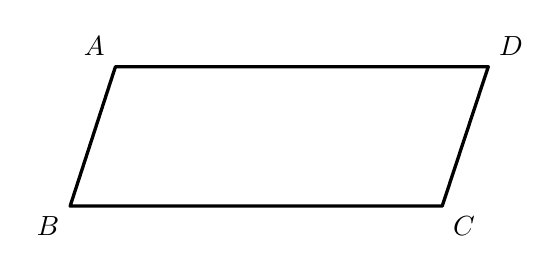
\begin{tikzpicture}[line width=1.2pt, line join=round]
  % Vertices: px -> TikZ with s=0.015, centre (232,91), y flipped
  \coordinate (A) at (-2.075,  0.885);
  \coordinate (D) at ( 2.660,  0.885);
  \coordinate (C) at ( 2.075, -0.885);
  \coordinate (B) at (-2.650, -0.885);

  % Trapezoid ABCD, solid black edges, no fill
  \draw[black] (A) -- (D) -- (C) -- (B) -- cycle;

  % Labels: A upper-left, D upper-right, C lower-right, B lower-left
  \node[above left]  at (A) {$A$};
  \node[above right] at (D) {$D$};
  \node[below right] at (C) {$C$};
  \node[below left]  at (B) {$B$};
\end{tikzpicture}
\end{document}